\documentclass[fire,article,submit,oneauthor,pdftex]{Definitions/mdpi} 

% MDPI internal commands
\firstpage{1} 
\makeatletter 
\setcounter{page}{\@firstpage} 
\makeatother
\pubvolume{1}
\issuenum{1}
\articlenumber{0}
\pubyear{2022}
\copyrightyear{2022}
\externaleditor{Academic Editor: Firstname Lastname} 
\datereceived{} 
\dateaccepted{} 
\datepublished{} 
\hreflink{https://doi.org/} % If needed use \linebreak

% Additional packages
\usepackage{longtable,booktabs}
\usepackage[utf8]{inputenc}

\usepackage{lmodern}

%=================================================================
% Full title of the paper (Capitalized)
\Title{Remote sensing in rangeland fire ecology: Comparing imagery to measured fire behavior, and burn severity across prescribed burns and wildfires}

% MDPI internal command: Title for citation in the left column
\TitleCitation{Remote sensing in rangeland fire ecology}

\newcommand{\orcidauthorA}{0000-0002-3763-7641} 

% Authors, for the paper (add full first names)
\Author{Devan Allen McGranahan $^{1,\dagger,}$\orcidA{} }

\firstnote{The US Department of Agriculture is an equal opportunity lender, provider, and employer. }


% Authors, for metadata in PDF
\AuthorCitation{McGranahan, D.A.}

% Affiliations / Addresses (Add [1] after \address if there is only one affiliation.)
\address{%
$^{1}$ \quad USDA Agricultural Research Service, Livestock \& Range Research Laboratory, Miles City, MT 59301 USA; Devan.McGranahan@usda.gov}

% Contact information of the corresponding author
\corres{Correspondence: \href{mailto:Devan.McGranahan@usda.gov}{\nolinkurl{Devan.McGranahan@usda.gov}}}

% Abstract (Do not use inserted blank lines, i.e. \\)
\abstract{Wildland fire scientists have made substantial advances in measuring fire behavior, but properly collecting data is often beyond the capacity of prescribed fire managers and by definition all but impossible for wildfire events. 
	While a method for the immediate assessment of burn severity has been developed around multispectral imagery from space-based Earth observation systems, there has been little comparison of these post-hoc metrics to actual fire behavior.
	Meanwhile, the application of research results from experimental prescribed burns to rangeland affected by wildfire can be impeded by a lack of understanding of how immediate burn severity  differs between wildfires and prescribed burns, especially in rangelands. 
	Overall, much of what is known about wildland fire behavior, severity, and effects comes from forests, whereas rangelands are characterized by having lower fuel loads comprised of fine vegetation that promotes high rates of spread and brief residence time. 
	This paper provides rangeland-specific information on the relationships between direct field-based fire behavior measurements and a space-based index of burn severity (differenced Normalized Burn Ratio, $\Delta$NBR, from Sentinel-2 imagery), and use those data to compare burn severity across 54 prescribed burns in North Dakota, USA, and 29 nearby wildfires in the US Northern Great Plains.
 	In prescribed burns, remotely-sensed burn severity increased with rate of spread and flame temperature 15 cm above the ground, but had no statistically-significant relationship with soil surface temperature. 
 	In the semi-arid western zone of the Northern Great Plains, wildfires and prescribed burns had similar, low-moderate severity; wildfires in the eastern zone tended to be moderately-high severity and thus greater than the low severity of the experimental prescribed burns. 
	 By describing meaningful gradients in surface fire behavior in rangelands with $\Delta$NBR, even those without the capacity to measure fire behavior in the field can monitor prescribed fire effectiveness and incorporate burn severity in adaptive management plans. 
	Understanding the relationship between burn severity across wildfires and prescribed burns is a critical step in applying knowledge gained from research on prescribed fires to areas impacted by wildfire. 
	Resistance to prescribed burning might be overcome by increasing livestock managers' experience with post-fire forage resources through grazing areas burned in unintentional wildfires, but current practice and policy dissuades or outright prevents ranchers from doing so.
	Future research ought to connect burn severity with ecosystem recovery metrics to ensure post-fire grazing does not impair rangeland sustainability. }

% Keywords
\keyword{Differenced Normalized Burn Ratio (dNBR), Rangeland fire ecology and management, Rate of spread, Thermocouple dataloggers, US Northern Great Plains, Wildland fire behavior }

\begin{document}

\section{Introduction}

Given the ubiquity of fire around the Earth and throughout its history, it is of little wonder that fire has had a primary role in human understandings of nature, shaping both the content and methods of natural philosophy and scientific investigations. 
From the four natural elements of Empedocles and Aristotle to Faraday's \emph{The Chemical History of a Candle}, the demystification of fire is emblematic of how Western civilization advanced from mythological to empirical ways of knowing \cite{pyne2016}. 
However, despite the efforts of reductionism, the scientific method, and controlled experimentation, a complete understanding of \emph{wildland fire}\textemdash combustion in its natural habitat, openly burning through vegetation\textemdash has remained elusive. 
While the essential contributions of each component in the fire triangle\textemdash heat, oxygen, and fuel\textemdash are broadly understood and can be tightly controlled in closed industrial environments, the degree of nuance in their dynamics in nature led Sullivan \cite[][p. 133]{sullivan2017} to describe wildland fires as ``a complex combination of highly chaotic chemical reactions and physical processes that continually and freely propagate through spatially-variable biomass fuels across variable terrain influenced by spatially and temporally varying atmospheric conditions.''

Wildland fire scientists use the term \emph{fire behavior} to describe energy release by the combustion of vegetation in terms of how fast fire moves, how much heat is released, and how long burning lasts \cite{mcgranahan2021a, finney2021}. 
Some of these are immediately observable\textemdash one can measure rate of spread simply by timing the passage of a flame front between points of a known distance apart; the length of a flame is related to energy release \cite{rothermel1980}. 
But each of these metrics require direct observation of the flame front, which is often precluded by smoke, lack of access, or the general danger to personnel posed by fire moving freely about. 
And while post-burn observations such as scorch height on trees can be used to infer intensity after the fact \cite{rothermel1980}, such methods have limited value in the rangeland ecosystems that cover approximately 54\% of the Earth's terrestrial surface and are characterized by having few if any trees \cite{ilri2021}. 

\subsection{Direct measurements of fire behavior} 

Several methods directly measure fire behavior beyond human line of sight. 
As a prominent property of fire is heat, wildland fire scientists have long tried to measure fire behavior as temperature.
For at least 75 years, measuring temperature in wildland fires has predominantly relied upon \emph{thermocouples}\textemdash pairs of two wires, composed of different metals, each of which transmit slightly different electric signals when their shared junction is heated; at the other end of the cable, differences in electrical properties across the two wires can be detected and converted to temperature \cite{vaartaja1949, engle1989,mcgranahan2020a, pavlasek2015, shannon2003}. 

Despite their ubiquity in wildland fire research, thermocouple systems have substantial limitations. 
Firstly, the physical limitations: \emph{e.g.}, response lags as the thermocouple material itself gains and loses heat from the material with which it is in contact, and  underestimations due to the fact the junction is losing heat to the ambient environment as well as absorbing it \cite{walker1968,lemaire2017}.  These errors are greatest when the temperature discrepancy between the junction and the media is greatest \cite{blevins1999}, which is exactly when flame fronts arrive at the sensor.
Finally, the junction retains heat even after the flame front passes and continues to register elevated temperatures; this post-fontal period is often erroneously interpreted as ``residual heating'' even when the media the junction is in contact with has returned to ambient temperature \cite{mcgranahan2020a}. 

\begin{figure}[t]
	\centering
	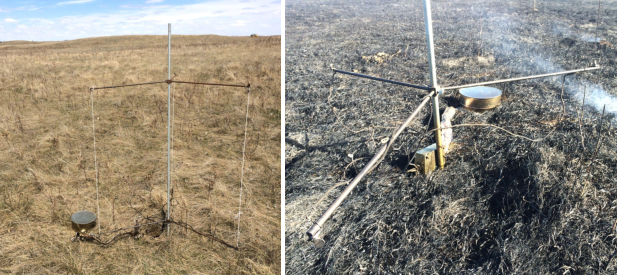
\includegraphics[width=1\columnwidth]{FeatherFlame.pdf}
	\caption{The FeatherFlame is an example of a thermocouple-based system designed to measure two-dimensional rate of spread, shown here deployed before a prescribed fire (left) and after the fire had passed (right). 
		The 1 m equilateral triangle holds three K-type thermocouples 15 cm above the soil surface. 
		Using the timestamps associated with flame temperatures recorded by the Arduino-based datalogger allows calculation of rate of spread through the array. 
		A fourth thermocouple is placed under litter at the soil surface. 
		The cylindrical galvanized cap protects the datalogger from heat, allowing \emph{in agris} fire behavior measurements.
	The system on the left is shown deployed with optional passive flame height sensors following \cite{finney1992}.   }
	\label{Fig:FeatherFlame} % Fig.~\ref{Fig:FeatherFlame}
\end{figure}

Secondly, even accurately measured temperature is a poor metric of fire behavior. 
Sensor placement has an outsized impact on temperature readings: the temperature of a single flame varies with distance from its base, and the vertical distribution of fuel can effect differences in the heating profile as great as whether temperatures increase or decrease with height away from the ground. 
Furthermore, recent work has called into question the decades-old concept that organisms have specific temperature mortality thresholds \cite{smith2016, pingree2019}; better is to quantify the total exposure of tissue to heat energy over time \cite{wright1970, dickinson2004, bova2005}.
Thus, Alexander \cite[][p. 350]{alexander1982} concluded, ``Measuring temperature merely introduces a cumbersome, secondary step in the study of fire effects when direct linkage to one or more fire-behavior characteristics would be more profitable,'' and Bova \& Dickinson \cite{bova2008} urge fire ecologists to move ``beyond fire temperatures.''

For many wildland fire scientists, rate of spread has become the most reliable metric of fire behavior\textemdash conceptually simple; relatively easy to observe, measure, and report; and a step towards calculating intensity, as an input in the Byram equation \cite{byram1959}. 
Rate of spread isn't perfect\textemdash it is affected by each component of the fire triangle but not singularly attributable to any, meaning several combinations of variables in the wildland fire environment can produce the same rate of spread \cite{finney2021}. 
But rate of spread is a common output in fire behavior prediction models \cite{perry1998, cruz2018}, particularly of head fires spreading with the wind. 
While such one-dimensional rate of spread is theoretically relatively easy to measure, especially during prescribed burns\textemdash stakes can be pre-positioned and a stopwatch used to time flame front travel between them\textemdash in reality, these measurements are challenged first by needing to ensure stakes are positioned perpendicular to the flame front, and second by needing to be within visual contact of the fuelbed ahead of the advancing fire.

Alternatively, measuring fire spread through a two-dimensional array of sensors has two advantages: it can be calculated regardless of the direction of spread, and does not need a human present \cite{finney2021}.
Thermocouple dataloggers can be used, but with the twist that the information of most value is the timestamp recorded when the flame front hits each sensor in the array: trigonometry can be applied to these arrival times to calculate the average speed at which the flame front moved through the array \cite[][Fig.~\ref{Fig:FeatherFlame}]{simard1982, simard1984, clements2019, mcgranahan2021, mcgranahan2023}. 

\subsection{Remote sensing in fire ecology} 

Beyond field-based measurements, space-based earth observation systems are increasingly being applied in wildland fire science \cite{szpakowski2019}. 
Fire ecologists have made particular use of the Normalized Burn Ratio (NBR), a multispectral product derived from Near-Infrared and Shortwave Infrared wavelengths, which have specific responses to reflectance changes caused by burning \cite{key2006a}. 
Changes effected by a specific fire event can be isolated by subtracting, or \emph{differencing}, post-fire NBR values from NBR values of the same point prior to the fire, creating a metric called Differenced Normalized Burn Ratio ($\Delta$NBR; Fig.~\ref{Fig:NBRexample}). 

\begin{figure}[t]
	\centering
	%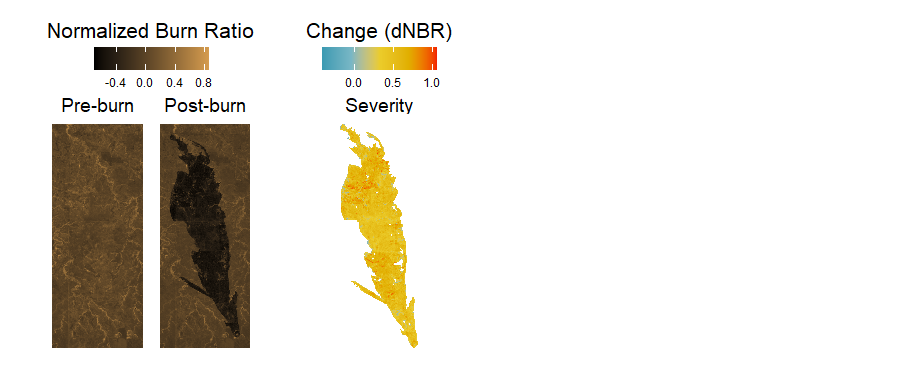
\includegraphics[width=1\columnwidth, trim={30 30 340 15},clip]	{example_wide.png} % left bottom right top
	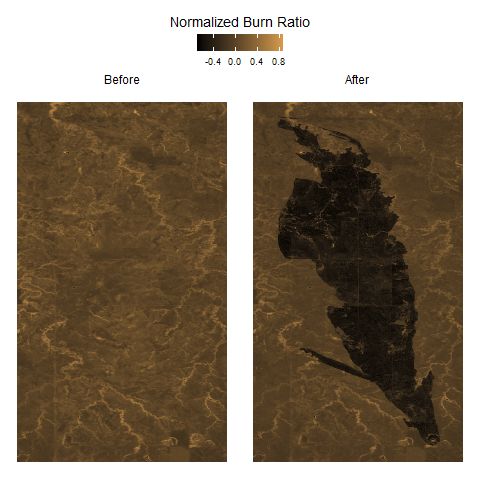
\includegraphics[width=0.72\columnwidth, trim={10 0 0 0},clip]{nbr_gg.png}~
	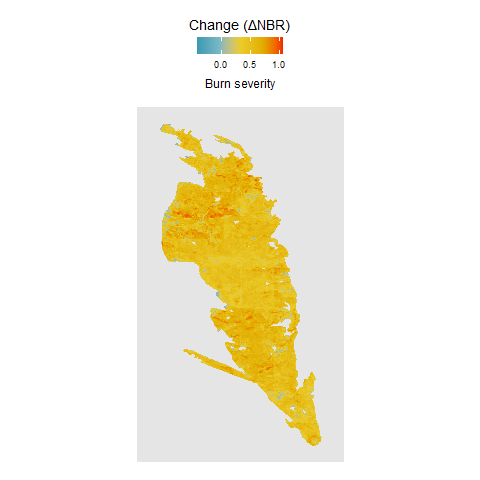
\includegraphics[width=0.28\columnwidth, trim={150 0 150 0},clip]{dnbr_gg.png}

	\caption{An example of a wildland fire from multipsectral imagery; 	see Fig.~\ref{Fig:TrueColor} for true color imagery, including a capture of the fire while it was burning.
		The longest axis of this fire extended 12 km (7.5 miles).
				\emph{Left:} The Normalized Burn Ratio for Before and After scenes from a fire in North Dakota, derived from Sentinel-2 Near-Infrared and Shortwave Infrared sensors.
		\emph{Right:} Burn severity is calculated as the difference between the Before and After NBR (Differenced NBR, or $\Delta$NBR), a measure of how much aboveground material the fire removed via combustion.
 }
	\label{Fig:NBRexample} % Fig.~\ref{Fig:NBRexample}
\end{figure}

Fire ecologists use $\Delta$NBR to estimate burn severity, defined in the context of interpreting remotely-sensed products as ``the degree of environmental change caused by fire \cite[][p. LA-6]{key2006a}.''
Temporal scale is a very important factor in the definition and interpretation of a $\Delta$NBR value. 
Generally speaking, burn severity assessments can be divided into \emph{extended} and \emph{immediate} \cite{key2006a,veraverbeke2010}.
The Monitoring Trends in Burn Severity program uses both imagery from immediately after a fire, to assess first-order effects on soil and vegetation consumption, and from the next growing season, to identify overall mortality to tree canopies in forests \cite{eidenshink2007a}.
The temporal distinction is particularly important in grasslands, where fire might remove all aboveground plant biomass down to mineral soil\textemdash by most definitions, high severity in an immediate assessment\textemdash but herbaceous plants have typically regrown by the end of the next growing season, which an extended assessment would classify as low severity \cite{lentile2006}. 

\subsection{Fire management in the 21\textsuperscript{st} century}
	
European colonization altered fire regimes around the world through top-down, command-and-control management that viewed wildland fire as destructive\textemdash and ironically, might have exacerbated the issue. 
As in many European and post-European nations, the United States had tight control over wildland fire by the middle of the 20\textsuperscript{th} century by suppressing unintentional ignitions and excluding intentional ignitions, especially cultural burning \cite{mcgranahan2021a, donovan2007}. 
But several ecosystems have been diagnosed with fire deficits in which the decades-long elimination of fire has had negative ecological effects and led to a buildup of vegetation biomass that drives high-intensity fires that are often uncharacteristically severe and difficult to control \cite{parks2015,kolden2019}. 
Management interventions often focus on fuel reduction through mechanical thinning or prescribed burning; conducted under less extreme conditions than wildfires typically occur, these ``good'' fires consume hazardous fuels without effecting high severity ot the rest of the ecosystem, and have shown varying degrees of effectiveness in reducing the severity of subsequent wildfires \cite{fernandes2003, brodie2024}. 

While the fire deficit affects most ecosystems in the United States, the prevalence of the ``good fire/bad fire'' duality has its origins in forests, with little critical examination of how or even whether it applies to rangelands. 
The colonial vanguard described a substantial amount of fire throughout the US Great Plains \cite{courtwright2007}, including the Northern Great Plains, specifically \cite{higgins1984,umbanhowar1996}. 
But colonization forced a transition from Indigenous fire use and native ungulates to a commercial ranching industry that relied upon grass being fed to cattle, not destroyed by fires \cite{courtwright2007}. 
Although this ethos is present today, especially in North Dakota \cite{boland2025}, a growing body of work demonstrates the benefits of prescribed fire for livestock production \cite{wanchuk2024, spiess2020, wanchuk2024a}. 
Even without active prescribed fire programs, a substantial portion of the Northwestern Great Plains already has a high incidence of fire\textemdash the ecoregion has one of the highest densities of wildfires in the US \cite{mcgranahan2024}. 
But there is a paucity of information on whether burn severity differs between prescribed burns and wildfires in the Northern Plains. 

\subsection{Objectives and hypotheses} 

The intent of this paper is two-fold: to provide rangeland-specific information on the relationships between direct field-based fire behavior measurements and space-based measurements of burn severity, and use those data to compare burn severity across prescribed burns and wildfires. 
Connecting remotely-sensed data to direct measurements helps calibrate assessments and monitoring programs that are unable to collect field-based fire behavior data but want insight into whether variation in remotely-sensed products has a meaningful relationship with ecological processes on the ground. 
Understanding how burn severity differs between prescribed burns and wildfires informs the transferability of ecological data on fire effects from burning experiments to broader landscapes affected by wildfire. 

The specific hypotheses tested here include: 
\begin{enumerate} 
	\item A positive linear relationship between field-based fire behavior and space-based burn severity metrics, as higher-intensity fires remove more aboveground plant material and expose more of the mineral surface to satellites.
	\item No difference in burn severity among wildfires and prescribed burns, as prescribed burns have been shown to demonstrate a wide range of burn severity that likely overlaps with that of wildfires \cite[e.g., ][]{mcgranahan2025}. 
\end{enumerate}

 
\section{Methods} 

\subsection{Study area}

The primary geographical scope of this study is the Northern Great Plains of the United States, specifically two experimental research locations in south-central and southwestern North Dakota (Fig.~\ref{Fig:StudyMap}). 
The south-central research location, referred to hereafter as the eastern location and in the eastern zone, is the North Dakota State University Central Grasslands Research Extension Center near Streeter, ND, located within the Northwestern Glaciated Plains in a relatively humid, mixed-grass prairie pothole landscape known as the Missouri Coteau. 

The southwestern research location, referred to hereafter as the western location and in the western zone, is focused around the North Dakota State University Hettinger Research Extension Center in Hettinger, ND, located within the semi-arid mixed-grass prairie of the Northwestern Great Plains. 
Research activities at the western location were conducted by North Dakota State University personnel on two blocks of Center-managed rangeland pastures within 5 km of the Center and another privately-owned ranch approximately 20 km to the east of Hettinger.

\begin{figure}[H]
	\centering
	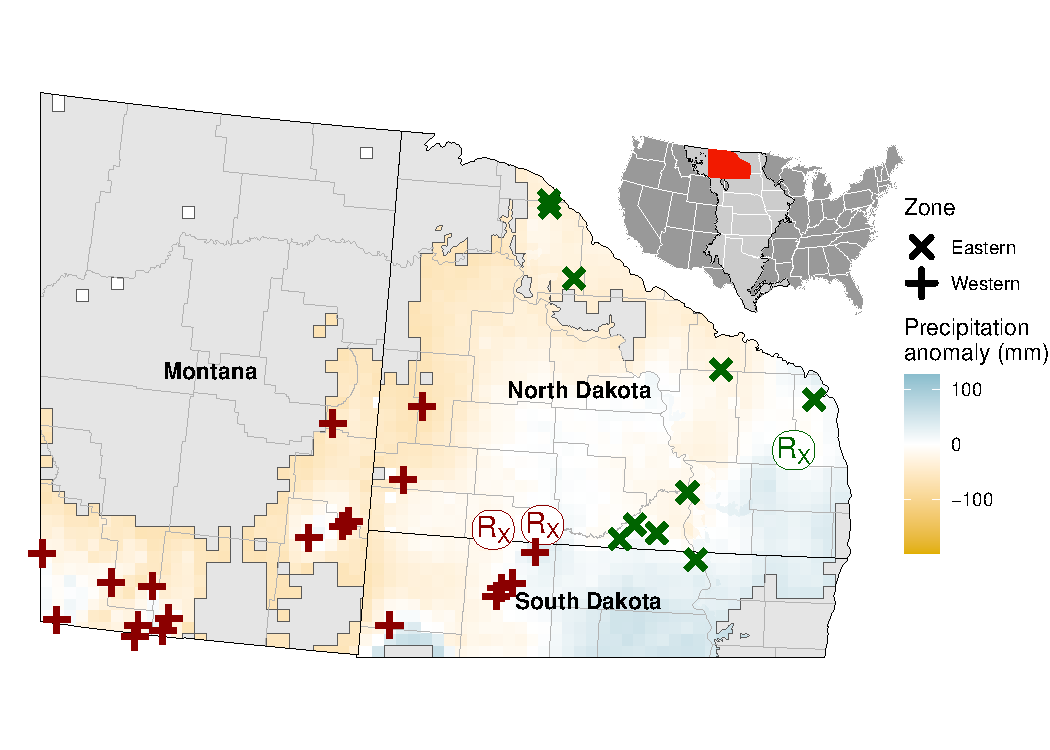
\includegraphics[width=1\columnwidth]{study_map-1.pdf}
	\caption{Location of rangeland research areas with experimental prescribed burns ($R_{X}$) and comparison wildfires ($\times$, $+$) in the Northern Great Plains. 
		Precipitation anomaly refers to the difference from mean annual precipitation at each of the western and eastern research locations for the study period (2017-2024); grey shaded areas have precipitation anomalies that exceed $\pm$ 3 standard deviations of mean annual precipitation and thus wildfires from these areas were excluded.
		Eastern and western zones align loosely with EPA Level III ecoregions NW Glaciated Plains and NW Great Plains, respectively (Fig.~\ref{AppFig:RegionMap}), with the exception of five wildfires near the Missouri River in south-central North Dakota being assigned to the eastern zone, which has substantially fewer wildfires than the western zone for comparison. 
		Inset: Study region within broader US Great Plains and continental US. }
	\label{Fig:StudyMap} %Fig.~\ref{Fig:StudyMap}
\end{figure}

\subsection{Data sources} 

This study reports on both prescribed burns conducted as part of rangeland ecology and management research, and wildfires that spread from unintentional ignitions in the region.
Data in this study are derived from two sources: fire behavior data collected \emph{in agris}\textemdash from field-based sensors recording temperature as prescribed fires occurred\textemdash and remotely-sensed products from space-based Earth observation satellites. 
Fire behavior data collected \emph{in agris} consist of flame front rate of spread, flame temperature, and soil surface temperature. 
Remotely-sensed data consist of immediate burn severity (differenced Normalized Burn Ratio, or $\Delta$NBR). 
Each of these data types and products are described below, and script for their processing and analysis in the \textsf{R} statistical environment \cite{rcoreteam2024} is freely available from Ag Data Commons \cite{mcgranahan2025b}.

\subsubsection{Location of fire incidents}

\textbf{Prescribed burns.\textemdash}54 individual experimental burn units were treated with prescribed broadcast burning between 2017 and 2020 by North Dakota State University personnel associated with the Hettinger (22) and Central Grasslands (32) Research Extension Centers. 
Burns were conducted as investigations into rangeland ecosystem responses to prescribed burning; results of this research and more extensive descriptions of experimental design have been published for both Central Grasslands \cite{duquette2022, wanchuk2024, mcgranahan2025a} and Hettinger \cite{spiess2024, spiess2025} Research Extension Centers. 
All burns at Central Grasslands and 15 at Hettinger were part of patch-burn grazing research in which 64 ha pastures were divided into four, 16 ha patches, one of which was burned annually. 
Burns at Central Grasslands were conducted in the spring (April\textendash May) and in the fall (October) at Hettinger using adaptive ignition strategies to maximize burned area within each unit, including ring, strip, and spiral ignitions. 
Seven additional fall burns at Hettinger were conducted on private ranch, with areas ranging from 5\textendash 12 ha \cite{mcgranahan2022}. 

\textbf{Wildfires.\textemdash}To compare burn severity effected by experimental prescribed burns to that produced by wildfires, a set of comparison wildfires were identified from the National Interagency Fire Center (NIFC) Interagency Fire Perimeter History\textemdash All Years geospatial database \cite{nifc2024}. 
Incidents in the database within the study region were filtered to wildfires of at least 10 ha that occurred between 2017\textendash 2024. 
As North Dakota had the fewest wildfire incidents in the region (Table~\ref{AppTab:StatesFires}), and very few occurred near the Research Extension Centers (Fig.~\ref{AppFig:RegionMap}), two additional steps were taken to provide sufficient sample size by extending beyond North Dakota while maximizing biophysical comparability with the prescribed burn locations:
 
Firstly, because wildfires spread across crop fields and pastures as well as through rangeland, the area within each wildfire perimeter identified as rangeland in the United States Forest Service (USFS) Extent of Coterminous US Rangelands raster layer \cite{usdaforestservicenodate} was summed, and incidents $<$20\% rangeland were excluded. 

Secondly, because the study area spans a wide precipitation gradient (Fig.~\ref{AppFig:RegionMap}) that effects substantial differences in fuel load and plant community composition, comparison wildfires were limited to those within 3 standard deviations of mean annual precipitation at the Research Extension Center in each zone (Fig.~\ref{Fig:StudyMap}).
Mean and standard deviation in annual precipitation for the period 2017\textendash 2024 were calculated from daily weather data collected by the respective North Dakota Agricultural Weather Network stations at each Center \cite{ndawn2025, ndawn2025a}. 
Precipitation anomalies across the study region were determined by creating a 10 $\times$ 10 km resolution grid and retrieving the mean annual precipitation, 2017\textendash 2024, for each cell centroid from the TerraClimate dataset \cite{abatzoglou2018}, accessed with the \emph{climateR} package \cite{johnson2021} for \textsf{R}. 
Centroids from wildfire perimeters were spatially joined with the nearest precipitation anomaly value in the grid, and incidents where the mean annual precipitation differed  by more than 3 standard deviations from that of the Research Extension Center in that zone were excluded.
Ten incidents were included as comparison wildfires in the eastern zone, and 19 in the western zone. 

Both prescribed burn and wildfire features were overlaid as polygons onto true color land surface imagery from the United States Geological Survey's National Map \cite{usgs_nm} to identify and exclude non-vegetated areas, such as ponds, areas of bare soil, and especially for wildfire perimeters, elements of the built environment such as farmsteads and petroleum well pads. 
As the NIFC perimeters often reflect general outlines of suppression efforts rather than boundaries of actual wildfire burned area, all perimeters were inspected visually over true color post-fire imagery and vertices edited for spatial accuracy.  

\subsubsection{Fire behavior data}

Field measurements of fire behavior were collected from 26 of the prescribed burns described above \cite{mcgranahan2022,mcgranahan2023}.
Briefly, fire behavior data were collected with K-type thermocouples (Omega Engineering, Inc., Norwalk, Connecticut, USA) attached to electronic data loggers using two different systems: 

Firstly, most prescribed burns (23) were sampled with the FeatherFlame system \cite{mcgranahan2021}, which consists of three thermocouples arranged in a 1m equilateral triangle 15 cm above the soil surface, and one thermocouple placed at the soil surface, all read by a single Arduino-based microcontroller writing temperature data at 1.5 Hz to a removable data storage card.
When arranged as such, the FeatherFlame system provides information on rate of spread, flame temperature at 15 cm, and soil surface temperature \cite{mcgranahan2022}. 
Nine FeatherFlame units were deployed in each of these 23 burns.

Secondly, fire behavior at three prescribed burns was measured with single-channel HOBO\textregistered~ U12 thermocouple dataloggers (Onset Computer Corporation, Bourne, Massachusetts, USA) logging at 1.0 Hz. 
At three sub-sample points within each burn, two loggers were deployed, one with a thermocouple placed at the soil surface and another at 15 cm above the soil surface. 
Rate of spread information was not available from these three instances of data from single-channel loggers. 

\subsubsection{Remotely-sensed data}

Burn severity\textemdash a measure of how much aboveground material was removed by wildland fire combustion\textemdash was calculated as the difference in Normalized Burn Ratio ($\Delta$NBR) from Normalized Burn Ratio (NBR) values in two images, the most-recent cloud-free image taken just before the burn, and the first cloud-free image taken just after the burn \cite[e.g.,][]{llorens2021}.
The NBR index is derived from the Near-Infrared and Shortwave Infrared bands \cite{key2006a}, and the subtraction of the NBR value in the post-burn image from the pre-burn NBR value at the same pixel provide $\Delta$NBR. 

NBR data were retrieved from the European Space Agency (ESA) Sentinel-2 mission's L2A collection, which provides multispectral imagery at 10 m $\times$ 10 m resolution from 2017 to present. 
All data were downloaded as geo-referenced raster files using the freely-available ESA Copernicus Browser, cropped to the bounding box of each visually-verified perimeter, generated with a custom EvalScript \cite{mcgranahan2025}, following visual inspection of each area of interest in true color images to ensure quality, cloud-free imagery. 

For the subset of prescribed burns with fire behavior measurements, the coordinates recorded when each datalogger was deployed were used to extract remotely-sensed data from the pre-burn and post-burn multispectral Sentinel-2 rasters using the \emph{terra} package for \textsf{R} \cite{hijmans2022}, to allow spatially-explicit tests of the relationship between \emph{in agris} measurements and remotely-sensed data at the finest scale available. 
For the broader comparison of prescribed burns and wildfires, each perimeter was reduced with an internal 20 m buffer (at least two raster cells in Sentinel-2 imagery) to minimize edge effects, and $\pm$100 gridded sample points were distributed within each perimeter. 
For wildfires, sampled pixels were limited to those identified as rangeland in the USFS product \cite{usdaforestservicenodate}. 
Remotely-sensed data were again extracted from the locally-downloaded multispectral rasters using \emph{terra}.

\subsection{Statistical analysis} 

Linear regression models were used to compare remotely-sensed burn severity against \emph{in agris} fire behavior data from prescribed burns, and to compare burn severity across prescribed burns and wildfires. 
In models comparing the 26 prescribed burns only, plot-level data from each experimental location were combined and fit with location and burn event as a nested random effect in linear mixed-effect models using  the \texttt{lmer} function in the \emph{lme4} package for \textsf{R} \cite{bates2015}. 
Statistical significance was determined with a $\chi^{2}$ test of deviance against null, intercept-only models. 

Models comparing burn severity across the 54 prescribed burns and 29 wildfires were fit with ordinary least squares regression using the \texttt{lm} function. 
These data were summarized as mean values for each unique fire event to eliminate pseudoreplication. 
Visual evidence suggested a likely statistical interaction between fire type and the two zones of the study area, which was confirmed by a significant interaction term in a global model fitting burn severity against fire type $\times$ zone.
Post-hoc comparisons of prescribed fires and wildfires within each zone were conducted with the \emph{emmeans} package \cite{lenth2018} by applying the \texttt{joint\_tests} function to the full model to produce an ANOVA table of test statistics for each zone. 

\section{Results} 

Remotely-sensed burn severity\textemdash as measured by differenced Normalized Burn Ratio ($\Delta$NBR)\textemdash increased with two directly-measured fire behavior responses (Fig.~\ref{Fig:SevBehav})\textemdash flame temperature ($\chi^{2}=$ 28.2, $P<$ 0.001) and rate of spread ($\chi^{2}=$ 4.3, $P=$ 0.04)\textemdash but burn severity had no statistically-significant relationship with soil surface temperature ($\chi^{2=}$ 2.0, $P>$  0.05). 

%Likewise, three fire response variables declined as fuelbed greenness (Normalized Differenced Vegetation Index, NDVI) increased (Fig.~\ref{Fig:BehavNDVI})\textemdash flame temperature ($\chi^{2}=$ 6.7, $P<$ 0.01), rate of spread ($\chi^{2}=$ 20, $P<$ 0.001), and burn severity ($\chi^{2}=$ 6.9, $P<$ 0.01)\textemdash but again there was no statistically-significant relationship with soil surface temperature ($\chi^{2}=$ 2.9, $P>$ 0.05). 

In the comparison of burn severity ($\Delta$NBR) across prescribed burns and wildfires in the two zones of the study region ( Fig.~\ref{Fig:WF_Rx}), there was a statistically-significant interaction between fire type and zone ($F_{1,79}=$ 10, $P<$ 0.01). 
In post-hoc pairwise contrasts, burn severity did not differ between prescribed burns and wildfires in the semi-arid western zone ($F_{1,79}=$ 1.5, $P>$ 0.05), but burn severity was statistically-significantly greater in wildfires that prescribed burns in the relatively higher-rainfall eastern zone ($F_{1,79}=$ 28, $P<$ 0.001). 

\begin{figure}[t]
	\centering
	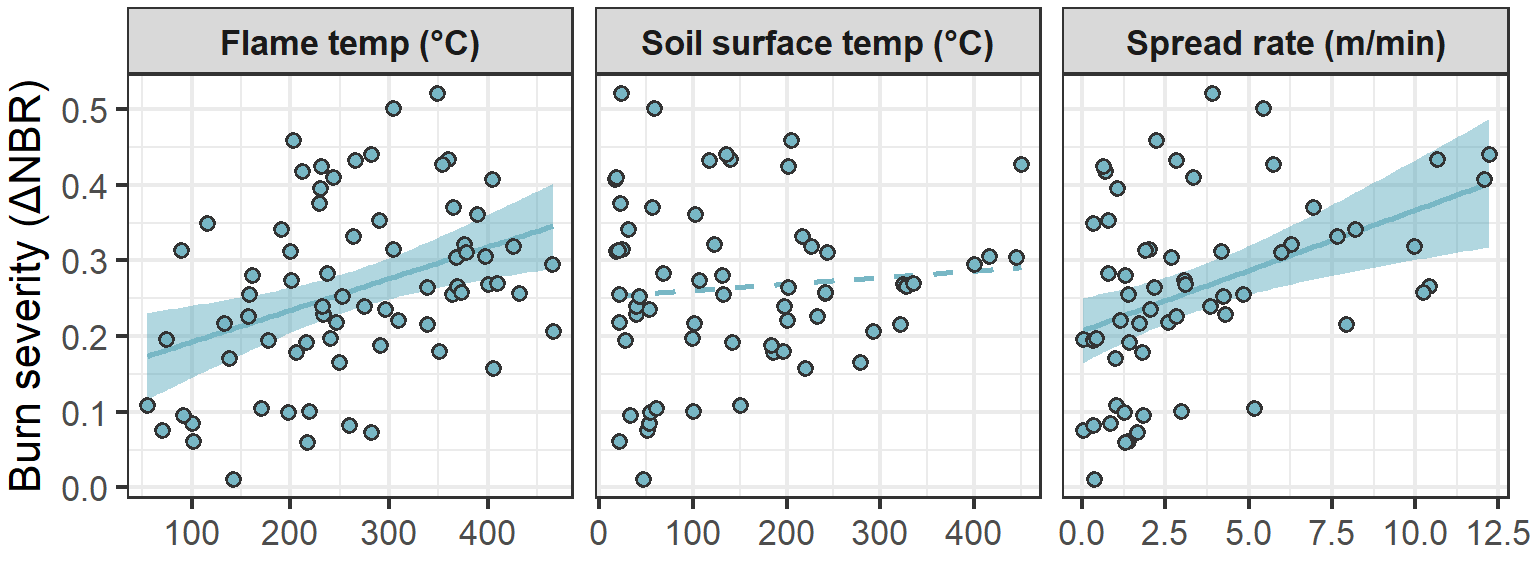
\includegraphics[width=1\columnwidth]{dNBR_v_FB-1.png}
	\caption{Burn severity\textemdash as measured by differenced Normalized Burn Ratio ($\Delta$NBR)\textemdash plotted against three fire behavior metrics measured during 26 prescribed burns in south-central and southwestern North Dakota.
	Solid trendlines with 95\% confidence intervals denote statistically-significant linear relationships in linear mixed-effect regression models.   }
	\label{Fig:SevBehav} % Fig.~\ref{Fig:SevBehav}
\end{figure}

%\begin{figure}[t]
%	\centering
%	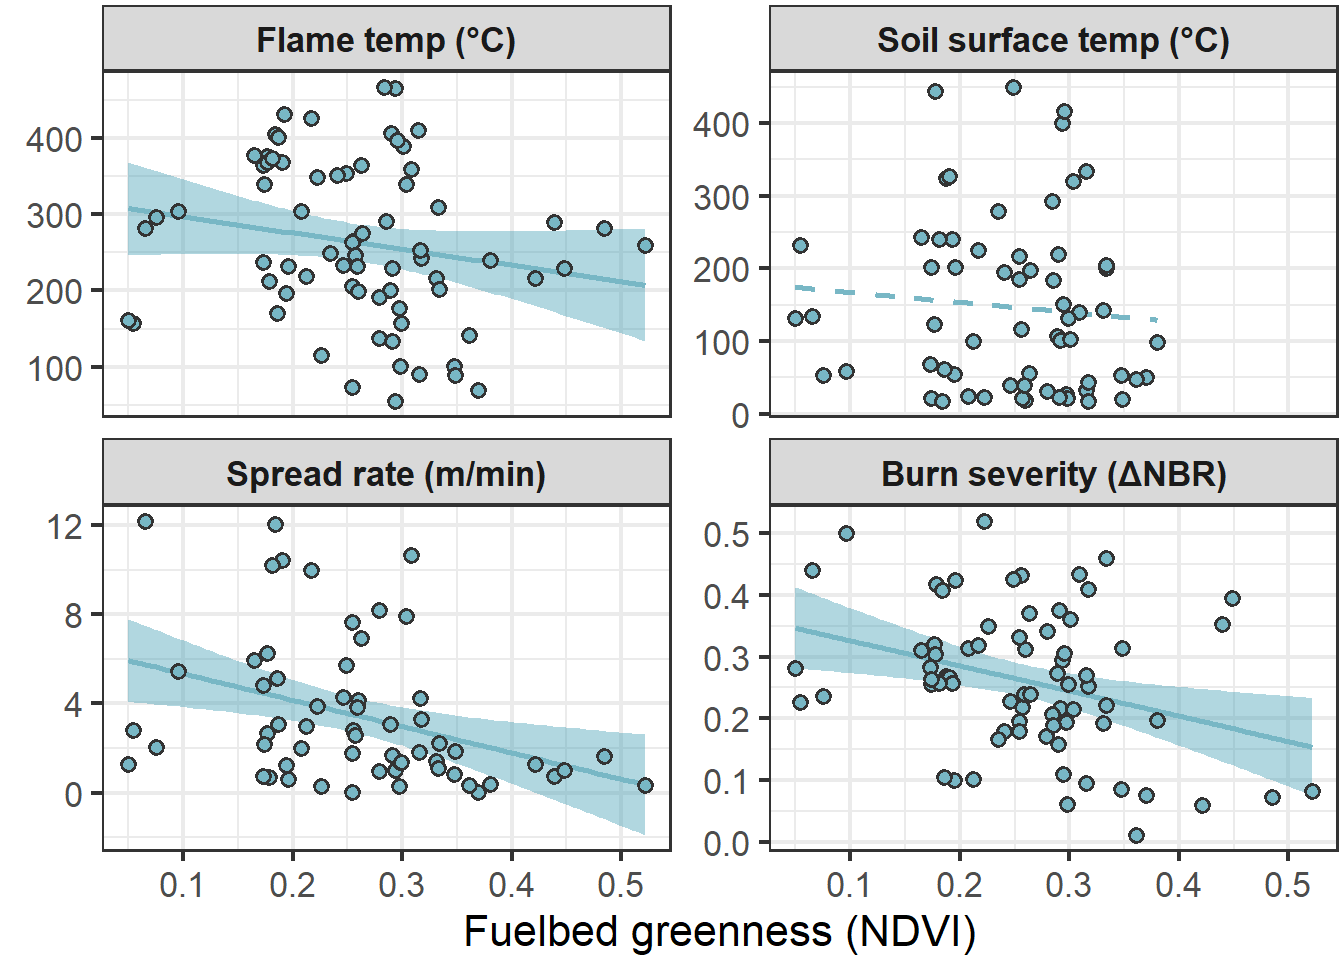
\includegraphics[width=1\columnwidth]{FB_v_ndvi-1.png}
%	\caption{Three field-sampled fire behavior metrics and a remotely-sensed measure of burn severity (differenced Normalized Burn Ratio, $\Delta$NBR) plotted against fuelbed greenness, measured as Normalized Difference Vegetation Index (NDVI) from the pre-burn Sentinel-2 image.
%		Solid trendlines with 95\% confidence intervals denote statistically-significant linear relationships in linear mixed-effect regression models.   }
%	\label{Fig:BehavNDVI} % Fig.~\ref{Fig:BehavNDVI}
%\end{figure}

\begin{figure}[t]
	\centering
	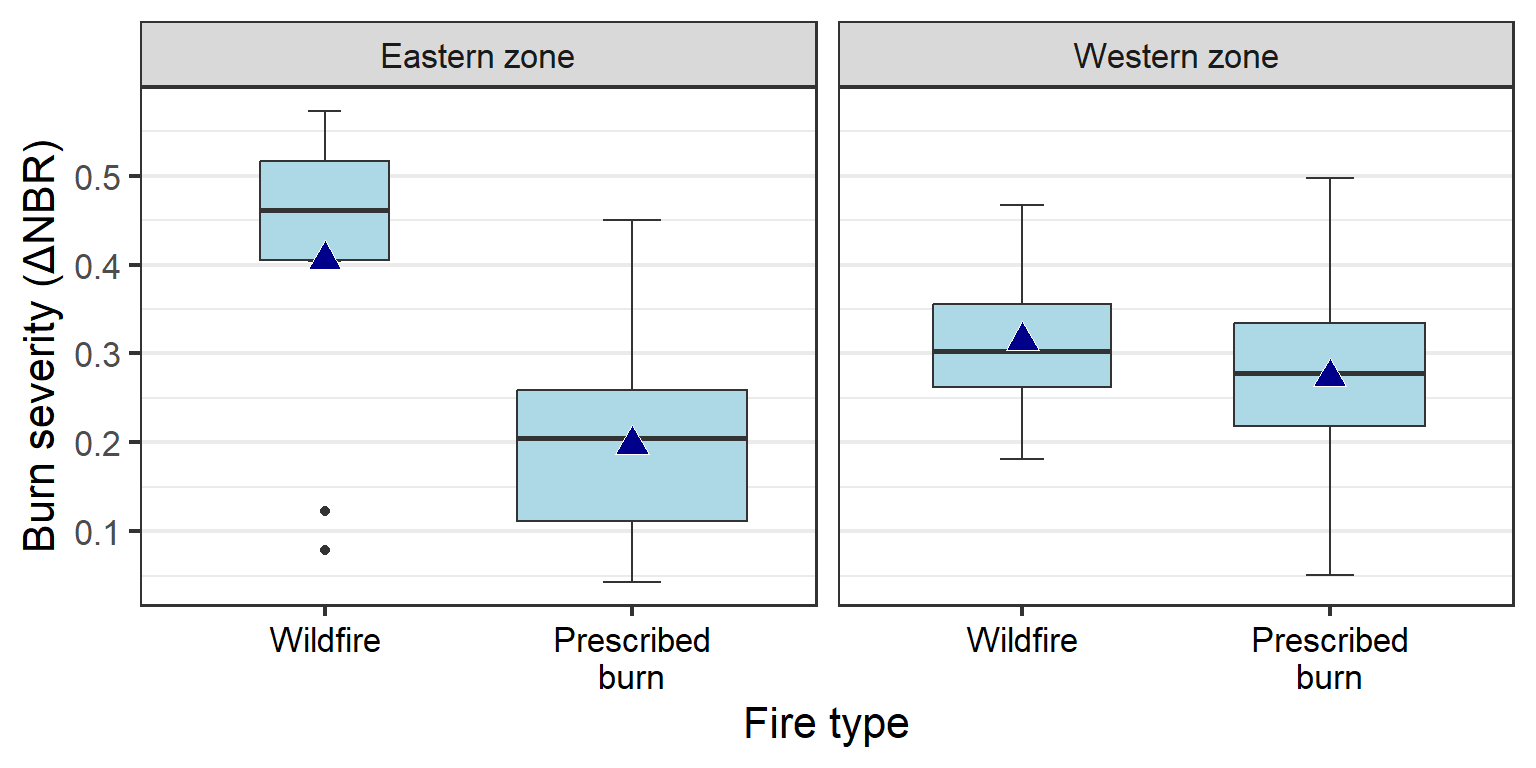
\includegraphics[width=1\columnwidth]{WF_v_Rx-1.png}
	\caption{Burn severity\textemdash as measured by differenced Normalized Burn Ratio ($\Delta$NBR)\textemdash across 29 wildfires and 54 prescribed burns in the two zones of the study region (see map, Fig.~\ref{Fig:StudyMap}). 
	Triangles represent group means. 
	Width of boxes scale with group sample size.   }
	\label{Fig:WF_Rx} % Fig.~\ref{Fig:WF_Rx}
\end{figure}

\section{Discussion} 

Using the US Northern Great Plains as a case study, this paper makes two primary comparisons that can support wildland fire scientists and managers in rangeland ecosystems worldwide. 
Firstly, three field-based fire behavior measurements (rate of spread, flame temperature, and soil surface temperature) from prescribed burns are compared to remotely-sensed burn severity (differenced Normalized Burn Ratio, $\Delta$NBR), and secondly, burn severity is compared between prescribed burns and wildfires. 
These comparisons provide partial support for each of two stated hypotheses: there is a positive linear relationship between remotely-sensed burn severity and measured flame temperature and rate of spread (but not soil surface temperature), and prescribed burn severity is not different from that effected by wildfires in the semi-arid western zone of the region (but wildfire severity is greater in the eastern zone). 

These results increase the range of options that provide insight into the variability of fire behavior and immediate fire effects in rangelands, facilitating better application of research from prescribed burns to areas affected by wildfire. 
Below are some considerations for both conventionally-collected and remotely-sensed data, and knowledge gaps that will require additional research to enhance the utility of these resources in wildland fire science and management applications.

\subsection{Remote sensing as complement, or even surrogate, to field-based measurements} 

Most apparently, managers unable to deploy fire behavior sensors during prescribed burns appear to be able to use freely-available remotely-sensed data on burn severity to describe meaningful gradients in fire behavior, and even those able to deploy sensors can use remotely-sensed data to describe fire behavior at  spatial scales beyond sample points. 
As such, remotely-sensed burn severity can enhance \emph{wildland fire science literacy}, the ability of scientists and managers to express and understand characteristics of the fire environment that give context for fire effects \cite{mcgranahan2018, mcgranahan2022a}. 
More specifically, rangeland fire ecologists can include summaries of burn severity alongside, or in lieu of, actual fire behavior measurements in their reports to help contextualize fire effects within a dose-response framework instead of a simple burned/unburned dichotomy \cite{smith2016a}. 

Although using time-temperature data from thermocouple dataloggers to calculate two-dimensional rate of spread is considered a more robust measure of wildland fire behavior than flame temperature alone, rate of spread is still an imperfect metric.
On one hand, rate of spread is a description of the wildland fire system, and does quantify specific physical processes within the fire environment \cite{finney2021}. 
Thus, some fire scientists measure responses such as total energy flux using radiometers to detect infrared radiation \cite{butler2004, kremens2012, obrien2018}, but such systems can be logistically challenging and expensive \cite{butler2010}. 

On the other hand, rate of spread is the initial output from several standard mathematical fire behavior prediction models \cite{rothermel1972,noble1980}, and is thus a useful connection between predicting and evaluating fire behavior. 
Rate of spread is also an input for equations that calculate fire intensity, the value of which ``lies not so much in the exact description of energy, but rather in the provision of numerical data for comparing fires \cite[][p. 354]{alexander1982}''. 
Knowing that burn severity scales with rate of spread adds a monitoring option for managers to use fire behavior prediction models as part of planning burns that meet specific objectives\textemdash and deciding under what conditions to conduct those burns effectively and safely. 

A particular concern with space-based multispectral products is a potentially coarser resolution than many processes within the fire environment and plant community play out. 
The inherent heterogeneity of wildland fuelbeds introduces variability in fire behavior that is critical to the survival of many species in fire-dependent ecosystems, such as how gaps between the vegetation that serves as wildland fuels reduce microsite fire intensity and thus severity to propagules \cite{daibes2018, atchley2021}. 
Analyses of post-fire patch dynamics suggest grain sizes\textemdash the finest scale of spatial independence\textemdash ranging from 0.5\textendash 10 m \cite{lamont1993, gimeno-garcia2004, pereira2013, gongalsky2016, moore2021}. 
But Sentinel-2 products are comprised of an average value for each 10 $\times$ 10 m pixel, and in the case of indices including NBR, one of the bands used in the calculations is collected at  20 $\times$ 20 m resolution. 
Thus, the pixel-scale averages in remotely-sensed severity data might obscure finer-scale instances of high severity that are ecologically meaningful to the individual organisms that comprise the broader-scale community. 
Research from forests suggest this might be more more of a concern for prescribed fires: Extreme fire weather conditions, more typical of wildfires, can override stand-level heterogeneity to effect more uniform severity \cite{romme2006, mcfarland2025}. 
In either case, remotely-sensed severity metrics should be compared to ecosystem-specific research on direct and indirect fire effects at the scale of relevant biological processes to determine how well severity indices correlate with rangeland fire effects, in addition to fire behavior. 

These data corroborate other evidence that the biotic and abiotic factors that typically have linear relationships with surface fire behavior metrics (\emph{e.g.}, rate of spread, flame properties) appear to have little correlation with soil heating. 
A subset of the prescribed burns included here were subject to a previous analysis of how fuel and fire weather conditions affected measured fire behavior, which reported that rate of spread increased with wind speed and flame temperature increased with fuel load and declined with fuel moisture; however, no fuel or weather factor had a statistically-significant effect on soil surface temperature \cite{mcgranahan2023}.
Likewise, this study showed no linear relationship between burn severity and soil surface temperature (Fig.~\ref{Fig:SevBehav}).
Similar patterns\textemdash or rather, lack thereof\textemdash between variables that drive rate of spread not correlating with soil surface temperature have been reported elsewhere \cite{gimeno-garcia2004}. 

The consistent lack of connections between the fire environment, soil heating, and burn severity suggest that at least for rangeland fuelbeds in which the primary carrier of fire is fine fuels (graminoids and herbaceous vegetation), a burned/unburned dichotomy might in fact be sufficient to explain first-order (direct) fire effects to soil. 
While it is certainly true that nutrient pools and microbial abundance are directly affected by soil heating, soil properties in rangelands recover within days or weeks of even relatively severe fires \cite{mcgranahan2022,docherty2012}; fungal communities are especially resilient to the low soil heating in grass-carried fires \cite{egidi2016}. 
The primary driver of belowground tissue damage is duration of heating; as such, fast-moving fires through grass-dominated fuelbeds effect the lowest amount of soil heating due to the shorter residence time of fine fuel combustion \cite{neary1999a, robichaud2000}. 
And because soil is a good insulator, even when soil surface temperatures in a subset of the prescribed burns here ranged from 200\textendash 400\textsuperscript{$\circ$}C, temperatures were consistently at or below 100\textsuperscript{$\circ$}C at depths of just 2 cm \cite{mcgranahan2022}. 

Thus, even intense fires through grass-dominated fuels might not exceed a threshold of soil heating to immediately effect anything beyond a general burned vs. unburned response pattern. 
However, second-order (indirect) effects to soil microbes might depend more on surface fire behavior\textemdash as modulated by abiotic and biotic conditions, and correlated with burn severity\textemdash because these organisms can be affected by post-fire soil conditions and plant community dynamics \cite{neary1999a}.

\subsection{Transferability of research from prescribed burns to wildfire-affected rangeland}

Although research on prescribed fire effects on rangeland plant communities has been conducted in the US Great Plains for over 100 years \cite{hensel1923, aldous1934, hulbert1969}, conceptions of wildfires and knowledge of their effects have largely been derived from forests \cite{crist2023}.
Due to the high potential fuel loading of forests (especially those under decades of fire deficit), there is a general concern that 'natural' and prescribed burns in forests are ecologically different \cite{williams1994}.  
But little scientific information substantiates such a difference in rangelands. 

As most rangeland ecosystems in the US are used for commercial livestock grazing, there is a general concern among managers throughout the western US about the impacts of livestock grazing on rangeland assumed to have been negatively affected by a wildfire. 
For example, the general guidance for the US Department of Interior Bureau of Land Management is to have their permittees defer, delay, or avoid altogether livestock grazing for up to two seasons on a grazing allotment burned by a wildfire \cite{blm2007}. 
While \citet{kluth2024} attribute the two-year convention to \citet{blaisdell1982}, it was more explicitly stated earlier, by \citet[][p. 9]{wright1979}: ``Prescribed fire can be a useful too in many big sagebrush communities if the fires are carefully planned and livestock do not graze the burn for two growing seasons.''
(Ironically, both sources were cautioning on the return of livestock to range recently treated with prescribed burns, a practice both \emph{recommended be used} to maintain herbaceous plant cover and reduce woody plants; the prescribed fire predicate has since been detached and the 2-year grazing exclusion adopted into pyro-skeptical wildfire management.)

It remains an open question whether rangeland management recommendations from the arid Great Basin region apply to semi-arid rangeland in the Northern Great Plains. 
Studying wildfire is difficult: by its very nature it occurs unpredictably, precluding the pre-treatment data collection that constitutes a robust sampling design, as simple burned-unburned comparisons are limited in their capacity to control for environmental and temporal variability \cite{zaitsev2016}. 
What research does exist on post-wildfire vegetation dynamics in the region suggests the caution over damage to plant communities is unjustified: productivity in the season after two wildfires in the Northwestern Great Plains was resilient to both wildfire and grazing \cite{gates2017, kral-obrien2020, williams2022}. 
Meanwhile, benefits of prescribed fire to the rangeland ecosystem and livestock grazing recent burns have been widely documented, especially from the prescribed fire experiments included in this study \cite{powell2018, spiess2024, mcgranahan2022, wanchuk2024, wanchuk2024a}.
What remains is an understanding of whether data from experimentally-controlled prescribed burns are relevant to wildfire incidents. 

The data presented here suggest that across both wildfires and prescribed burns, burn severity in the Northern Great Plains is generally low to moderate, especially in the western zone; wildfires in the more humid eastern zone tend to be moderately high (Fig.~\ref{Fig:WF_Rx}).
Based on the lack of difference in burn severity between wildfires and prescribed burns in semi-arid rangeland of the Northwestern Great Plains, it is likely that research results from prescribed burns in the region are applicable to ecologically-similar areas affected by wildfire. 
Although less certain, there is possibly a useful degree of transferability between prescribed burn research and wildfires in the eastern zone as well, because despite the statistically-significant difference in burn severity, even the incidents with the most severe burns fall below the 0.66 $\Delta$NBR threshold for high burn severity \cite{key2006a}. 

Consistently low to moderate burn severity aside, a number of biotic and abiotic differences between most wildfires and prescribed burns ought to be resolved before the ecological effects of these fires can be considered consistent, as well. 
Many of these differences fall under the general umbrella of seasonality, which affects both the conditions of the fire environment and the biological status of organisms impacted by heating, \emph{e.g.} seasonal phenology and dormancy considerations. 
A common denominator of weather conditions conducive to burning relate to moisture: dry air from cold fronts, dry surface conditions from periods with little to no precipitation, and low relative humidity \cite{flannigan2001}. 
Additional factors include fuel load and wind speed at the time of an ignition further modulate energy release \cite{cheney1995, reid2010, kidnie2015, gomes2020}.

Prescribed burn operations are typically reserved for seasons more conducive to manageable fire behavior, while wildfires occur whenever fuels and weather align with ignitions. 
In the eastern zone, prescribed burns reported here were conducted entirely in April and May, whereas the wildfires in the  eastern zone included here occurred fairly consistently between January and August (Table~\ref{AppTab:FireMonths}). 
Prescribed burns in the western zone were restricted to October, whereas all wildfires included here occurred January-September, and mostly in July and August (Table~\ref{AppTab:FireMonths}). 
And then within seasons, prescribed burns are often only conducted under moderate weather conditions, which likely accounts for substantially lower burn severity in experimental prescribed fires in the eastern zone: for instance, prescribed burns at the Central Grasslands Research Extension Center were only conducted on days with wind speeds below the 42-yr median \cite{mcgranahan2025}. 
Future research should measure post-fire effects on soils and plants on wildfires, as well, to determine that seasonal differences do not limit ecosystem recovery beyond that observed after prescribed burns despite consistent low to moderate severities in immediate assessments based on remotely-sensed data. 

\subsection{Conclusion}

These data suggest wildland fire professionals can describe meaningful gradients in surface fire behavior in rangelands within an immediate assessment framework using differenced Normalized Burn Ratio ($\Delta$NBR) from remotely-sensed imagery as a metric of burn severity. 
Thus, even those without the capacity to measure fire behavior in the field can monitor prescribed fire effectiveness and incorporate burn severity in adaptive management plans. 
Understanding the relationship between burn severity across wildfires and prescribed burns is a critical step in applying knowledge gained from research on prescribed fires to areas impacted by wildfire. 
Resistance to prescribed burning might be overcome by increasing livestock managers' experience with post-fire forage resources through grazing areas burned in unintentional wildfires, but current practice and policy dissuades or outright prevents ranchers from doing so.
Despite the know improvements to forage, it is essential that future research study the association between burn severity with ecosystem recovery metrics to ensure post-fire grazing does not impair the sustainability of rangeland ecosystems. 


\vspace{6pt}

\acknowledgments{The prescribed fires reported here depended on efforts of several North Dakota State University faculty and graduate students, especially Kevin Sedivec and Ben Geaumont for location management and equipment; and Megan Wanchuk, Jonathan Spiess, and Megan Zopfi (University of North Dakota) for their efforts in fire behavior data collection. 
Jay Angerer provided expertise for many aspects of remotely-sensed data management. }

\authorcontributions{DA McGranahan did everything related to this paper. }

\conflictsofinterest{The author declares no conflict of interest.}

\dataavailability{Data for formal analysis, modified perimeters of included wildfires, and script are freely available on Ag Data Commons \cite{mcgranahan2025b}. }

\funding{No specific funding was acquired for this study.}

\appendixtitles{yes} 
\appendixstart
\appendix
 \section{Additional information}

\begin{figure}[H]
	\centering
	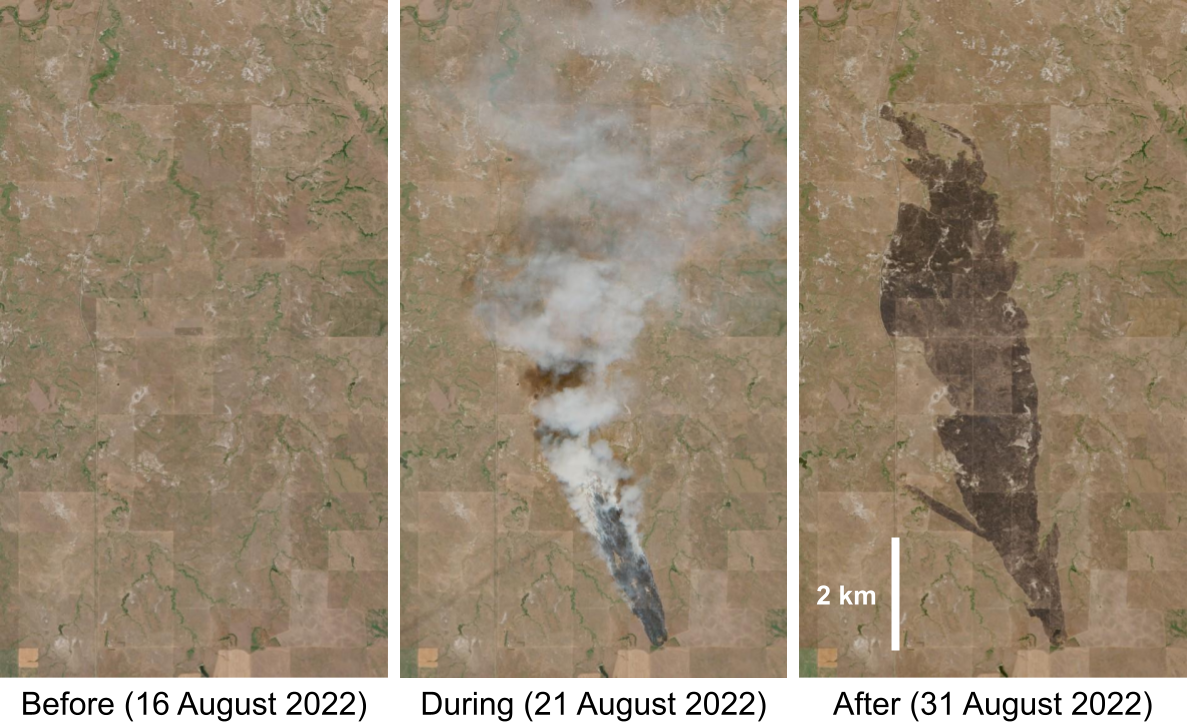
\includegraphics[width=1\columnwidth]{SatelliteFireSpread.png}
	\caption{True-color images of a fire in North Dakota, which a satellite from the Sentinel-2 mission caught shortly after the fire started\textemdash a tall smoke plume coming off the wind-driven head fire is clearly visible on August 21, 2022.
	NBR and $\Delta$NBR in Fig.~\ref{Fig:NBRexample}.  }
	\label{Fig:TrueColor} % Fig.~\ref{Fig:TrueColor}
\end{figure}

\begin{figure}[H]
	\centering
	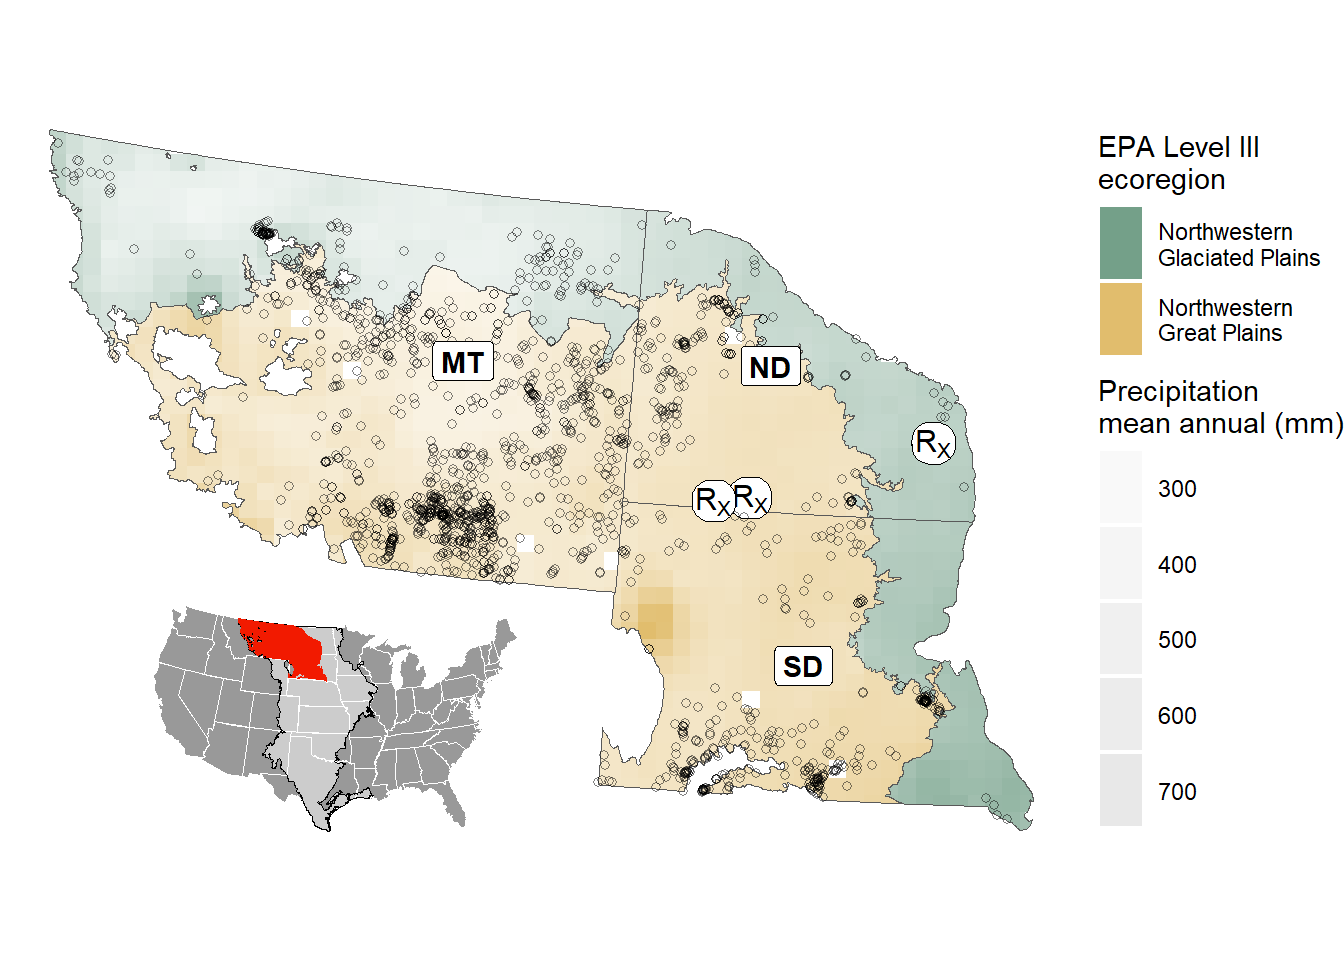
\includegraphics[width=1\columnwidth]{region_map-1.png}
	\caption{Portions of Montana, North Dakota, and South Dakota encompassed by the primary EPA Level III ecoregions of the Northern Great Plains\textemdash Northwestern Glaciated Plains and Northwestern Great Plains\textemdash within the broader US Great Plains (inset, red area). 
	Ecoregions shaded by mean total annual precipitation for the complete years in the study period (2017\textendash 2024). 
	$R_{x}$ badges indicate locations of prescribed burn experiments. 
	Open circles denote centroids of wildfire events in the NIFC Interagency Wildfire Perimeter database, 2017-2023; total counts presented in Table~\ref{AppTab:StatesFires}. }
	\label{AppFig:RegionMap} % Fig.~\ref{AppFig:RegionMap}
\end{figure}

\begin{specialtable}[H] 
\caption{Summarized totals of wildfire incidents presented in Fig.~\ref{AppFig:RegionMap}.  }
\label{AppTab:StatesFires}
\begin{tabular}{p{3cm}p{4cm}p{3cm}p{1cm}}
\toprule
\textbf{State} & \textbf{NW Glaciated Plains} & \textbf{NW Great Plains} & \textbf{Total} \\ 
\hline
 Montana (MT) & 153 & 998 & 1151 \\ 
South Dakota (SD) &   9 & 339 & 348 \\ 
North Dakota (ND) &  21 & 150 & 171 \\
\hline
\bottomrule
\end{tabular}
\end{specialtable}

\begin{specialtable}[H] 
	\caption{Monthy distribution of the wildfire subset used in this study, by zone, as determined by midpoint of pre- and post-fire image dates.  }
	\label{AppTab:FireMonths}
\begin{tabular}{lccccccccc}
	\hline
	Zone & Jan & Feb & Mar & Apr & May & Jun & Jul & Aug & Sep \\ 
	\hline
	East &   1 &  1 &   1  &   2 &  2 & 0   & 2 &  1 & 0  \\ 
	West &   1 &  0 &   2 &   3 &  0  & 0   & 5 &  6 &  2 \\ 
	\bottomrule
	\end{tabular}
\end{specialtable}



\end{paracol}

\reftitle{References}
\externalbibliography{yes}
\bibliography{RemoteSensingFireBehavior.bib}


\end{document}
